\chapter{Einleitung}
\label{sec:einl}
Das High-Performance-Computing (HPC) besch\"aftigt sich mit dem Hochleistungsrechnen. Im Bereich des High-Performance-Computing geht es darum, dass Computer mit m\"oglichst grosser Leistung und \"moglichst vielen parallelen Prozessen operieren. Dabei ist es unerl\"asslich, dass zum einen CPU-Berechnungen als auch Speicher-Zugriffe m\"oglichst schnell durchgef\"uhrt werden k\"onnen.
\section{BWHPC}
Die Arbeiten in diesem Projekt werden am Hochleistungscluster BWHPC durchgef\"uhrt. Das BWHPC ist ein Hochleistungscluster des Landes Baden W\"urttemberg, welcher an der Universit\"at Karlsruhe steht und f\"ur Forschungszwecke eingesetzt wird.
\section{Mooresches Gesetz}
Die Leistung von Prozessoren wird immer schneller. Die Gewschwindigkeit des Wachstums kann durch das sog. Mooresche Gesetz beschrieben werden. Die Definition dieses Gesetzes ist im folgenden gegeben.

\begin{quote}Die Anzahl an Transistoren, die in einen integrierten Schaltkreis festgelegter Gr\"osse passen, verdoppelt sich etwa alle zwei Jahre.~\cite{Schanze.25.02.2016}\end{quote}
Das Mooresche Gesetz sagt im Umkehrschluss also aus, dass sich die Prozessorleistung etwa alle zwei Jahre verdoppelt. Dieses Wachstum ist in Abbildung \ref{fig:moore} f\"ur Intelprozessoren beispielhaft dargestellt.

\begin{figure}[h]
	\centering
	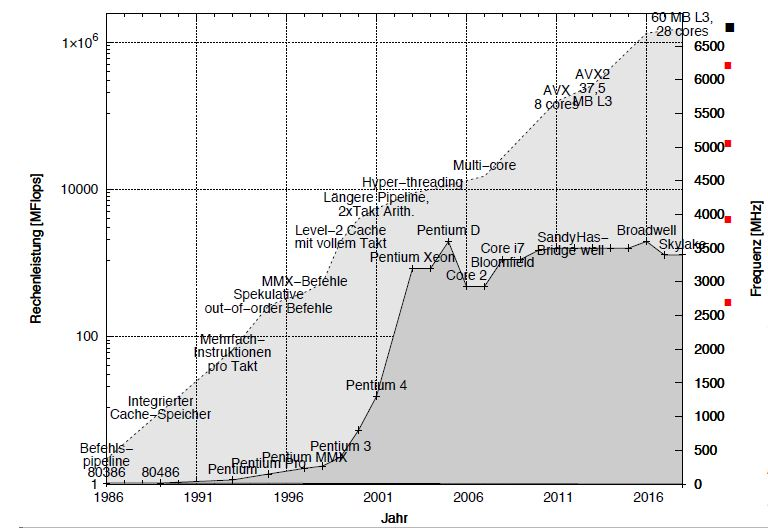
\includegraphics[width=7cm]{fig/moore.JPG}
	\caption{Mooresches Gesetz}
	\label{fig:moore}
\end{figure}
Auffallend in Abbildung \ref{fig:moore} ist, dass die Frequenz der einzelnen Kerne seit einigen Jahren nicht mehr zunimmt. Dies bedeutet, dass das Wachstum nicht mehr durch das Steigern von Leistung, sondern durch das Parallelisieren von CPU-Kernen bestimmt wird. Ein neuer Prozessor hat also nicht mehr Leistung als ein \"älterer, sondern er besteht aus mehr CPU-Kernen. Gerade im Bereich des Hochleistungsrechnen ergibt sich daraus, dass viele Anwendungen parallel ausgef\"uhrt werden.
\section{Speicherzugriffe}
Mit Speicherzugriffen kann ein Prozessor Daten aus einem Speicher holen und auch in ihn schreiben. Dabei kann im Wesentlichen zwischen Registern, Caches, Hauptspeicher und Festplatte unterschieden werden. Wohingegen der Zugriff auf Register ohne grosse Latenzen m\"oglich ist, ist der Zugriff auf andere Speicher deutlich langsamer. Die Zugriffszeiten sind in Tabelle \ref{tab:Speicher} vergleichend dargestellt. Faktor 10 bedeutet hierbei, dass die CPU 10 mal schneller als der Zugriff auf den L3-Cache ist. 
\begin{table}[h]
	\centering
	\begin{tabular}{l|l}
		\textbf{Speicher} & \textbf{Zugriffszeit} \\
		\hline
		CPU zu L3-Cache & Faktor 10 \\
		\hline
		CPU zu Hauptspeicher & Faktor 100 bis 1000 \\
		\hline
		CPU zu Festplatte & Faktor 1000 bis 1000000 \\
	\end{tabular}
	\caption{Speicherzugriffe}
	\label{tab:Speicher}
\end{table}

Aufgrund dieser Geschwindigkeitsunterschiede ist es notwendig den Zugriff auf Speicher m\"oglichst effizient zu gestalten, da es sonst zu erheblichen Engp\"assen in Programmabl\"aufen kommen kann.

\section{Dateisysteme}
Der Zugriff auf Dateien, welche auf der Festplatte liegen, geschieht \"uber Dateisysteme. Mit einem Dateisystem wird dabei die Ablage dieser Dateien auf der Festplatte organisiert. Damit k\"onnen diese dann gespeichert, gelesen, ver\"andert oder ge\"loscht werden.
Beim Zugriff auf Dateien kann im Wesentlichen zwischen seriellem und parallelem File-IO unterschieden werden. Die Unterscheidung hierbei liegt darin, wie parallel ausgef\"uhrte Programme auf Dateien zugreifen.
\subsection{Serieller IO}
Beim seriellen IO l\"auft der komplette IO \"uber einen Masterprozess. Dies bedeutet, dass Programme nicht gleichzeitig auf eine Datei zugreifen k\"onnen. Dies ist in Abbildung \ref{fig:serial} ersichtlich.
\begin{figure}[h]
	\centering
	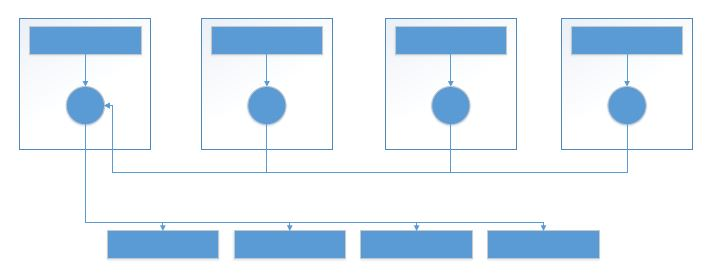
\includegraphics[width=7cm]{fig/SerialIO.JPG}
	\caption{Serial IO \cite{Cazes.26.09.2013}}
	\label{fig:serial}
\end{figure}

In Abbildung \ref{fig:serial} ist zu erkennen, dass es zu starken Engp\"assen kommen kann, wenn mehrere Programme gleichzeitig auf eine Datei zugreifen wollen. Diese Art des IO stellt daher auf kleinen Desktop-Computern mit nur wenigen parallelen Programmen kein Problem dar, im Bereich des High-Performance-Computing mit vielen parallelen Programmen sollte aber auf andere Methoden zur\"uckgegriffen werden.\cite{Cazes.26.09.2013}

\subsection{Paralleler IO}
Im Gegensatz zum seriellen IO ist es beim parallelen IO m\"oglich, dass mehrere Prozesse zeitgleich auf eine Datei zugreifen k\"onnen. Dies ist in \ref{fig:parallel} dargestellt. Darin wird ersichtlich, dass der IO nicht mehr \"uber einen Masterprozess l\"auft, sondern, dass die einzelnen Prozesse ihren IO unabh\"angig voneinander durchf\"uhren.
\begin{figure}[h]
	\centering
	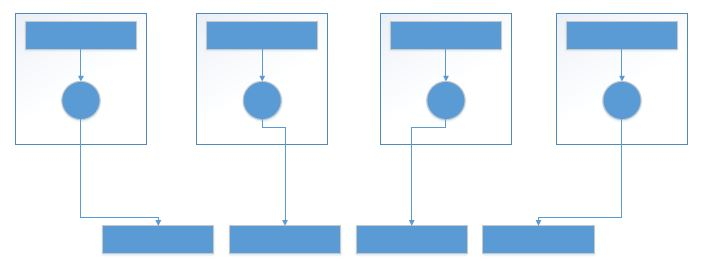
\includegraphics[width=7cm]{fig/ParallelIO.JPG}
	\caption{Parallel IO \cite{Cazes.26.09.2013}}
	\label{fig:parallel}
\end{figure}
Der Vorteil hierbei liegt darin, dass die einzelnen Prozesse parallel auf Dateien zugreifen bzw. in diese schreiben k\"onnen. Gerade im Bereich des High-Performance-Computing mit sehr vielen parallelen Prozessen stellt dies einen wichtigen Vorteil dar.\cite{Cazes.26.09.2013}
\subsection{POSIX IO}
POSIX-IO ist der IO-Part des POSIX-Standards. Der POSIX-Standard ist ein Standard f\"Ur die Kommunikation von Prozessen mit dem Betriebssystem. POSIX-IO beschreibt dabei verschiedene Funktionen, \"uber welche Programme in einem POSIX-Betriebssystem auf Dateien zugreifen k\"onnen. Mit diesen Funktionen kann ein Programm dann bspw. eine Datei \"offnen, in diese schreiben und diese anschliessend wieder schliessen. Der Zugriff auf POSIX-IO-Funktionen geschieht zumeist \"uber die Glibc. Die Glibc ist eine Bibliothek, welche Systemaufrufe als C-Funktionen bereitstellt. \"Uber diese C-Funktionen k\"onnen Programme dann Systemaufrufe durchf\"uhren.\newline POSIX-IO eignet sich gut f\"ur den Einsatz im Bereich von Desktop-PCs mit nur vergleichsweise wenigen parallelen Prozessen. F\"ur den Einsatz im HPC-Bereich hat POSIX-IO jedoch einige Schwachstellen, welche im Folgenden erl\"autert werden sollen.
\subsubsection{Metadaten}
Dateien auf einem POSIX-Dateisystem m\"ussen eine Vielzahl an Metadaten besitzen. Sollen Informationen \"uber eine Datei angezeigt werden, m\"ussen diese Metadaten ausgelesen werden. Auf HPC-Systemen kann dies einen Nachteil darstellen, da das Auslesen der Metadaten von vielen Dateien mitunter sehr lange dauert\cite{Layton.02.03.2010}.\newline
Ein weiterer Nachteil der Metadaten liegt darin, dass diese bei jedem Schreibvorgang aktualisiert werden m\"ussen. Dies kostet sehr viel Zeit, wodurch Schreibvorg\"ange in Bezug auf die Geschwindigkeit erheblich eingeschr\"ankt werden.\newline
Dar\"uber hinaus sind die Metadaten in POSIX-IO sehr unflexibel, da s\"amtliche Dateien alle Metadaten besitzen m\"ussen und nicht bspw. Metadaten f\"ur alle Dateien in einem Ordner gelten k\"onnen.
\subsubsection{File-Descriptoren}
Bevor eine Datei in POSIX gelesen werden kann, muss diese zun\"achst ge\"offnet werden, um einen File-Descriptor zu erhalten. In diesem File-Descriptor wird der Status der Datei gespeichert. Wird eine Datei wieder geschlossen, wird der File-Descriptor wieder freigegeben.\newline
Der Nachteil von File-Descriptoren kommt zum Tragen, wenn viele Prozesse gleichzeitig auf ein Dateisystem zugreifen wollen. Dann muss das Betriebssystem sehr viele File-Descriptoren parallel verwalten, wodurch bspw. das \"Offnen einer Datei immer langsamer wird, je mehr Prozesse parallel auf das Dateisystem zugreifen. In Abbildung \ref{fig:posix} ist dabei ersichtlich, dass das \"Offnen einer Datei linear langsamer wird, je mehr parallele Prozesse auf das Dateisystem zugreifen.
\begin{figure}[h]
	\centering
	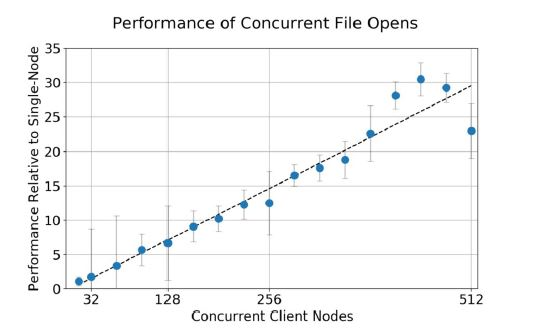
\includegraphics[width=7cm]{fig/PosixIO.JPG}
	\caption{\"Offnen einer Datei bei POSIX-IO \cite{Lockwood.11.09.2017}}
	\label{fig:posix}
\end{figure}
\subsubsection{Konsistenz}
Das Schreiben in eine Datei muss in POSIX konsistent sein. Dies bedeutet, dass das Schreiben die Ausf\"uhrung einer Applikation so lange blockiert, bis sichergestellt ist, dass ein Lesezugriff das neu geschriebene sieht. Dies hat wiederum den Nachteil, dass im Ausführen von Applikationen durch das Schreiben in eine Datei starke Latenzzeiten entstehen. Im HPC-Bereich mit vielen parallelen Applikationen stellt dies ein grosses Problem dar, wenn viele Prozesse gleichzeitig in Dateien schreiben wollen.
\cite{Lockwood.11.09.2017}
\subsection{MPI-IO}
MPIO-IO ist der IO-Part des Message Passing Interface (MPI). MPIO-IO ist dabei eine sog. Middleware, welche i.d.R. nicht direkt von Anwendungen sondern nur indirekt durch h\"ohere Schichten genutzt wird. Es definiert somit einen Standard f\"ur parallele IO-Operationen in einer MPI-Applikation. Im Gegensatz zu POSIX-IO ist der Zugriff auf Dateien hierbei nicht Bytestrom- sondern elementorientiert. Der Aufbau einer Datei in MPI-IO ist in Abbildung \ref{fig:dateityp} und in Abbildung \ref{fig:dateisicht} ersichtlich. Eine Datei wird dabei in sog. Fliessen aufgeteilt. Auf diese Fliessen kann \"uber einen Dateityp zugegriffen werden. Ein Dateityp beschreibt ein Muster an Fliessen, welches sich \"uber Teile der Datei oder \"uber die ganze Datei wiederholt. Ein solches Muster ist in Abbildung \ref{fig:dateityp} dargestellt. Jede Fliesse im Muster besteht wiederum aus einem elementaren Typ. Der elementare Typ ist der Datentyp \"uber welchen auf die Datei zugegriffen werden kann. Ein Prozess, der auf die Datei \"uber diesen Dateityp zugreift kann somit auf alle Fliessen zugreifen, welche in diesem Muster liegen.


\begin{figure}[h]
	\centering
	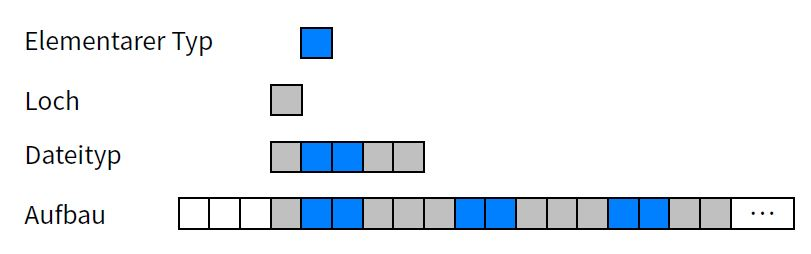
\includegraphics[width=7cm]{fig/Dateityp.JPG}
	\caption{Dateityp bei MPI-IO \cite{Kuhn.13.05.2016}}
	\label{fig:dateityp}
\end{figure}

In Abbildung \ref{fig:dateisicht} ist der Aufbau einer Datei aus Sicht von Prozessen dargestellt. Dies wird auch als Dateisicht bezeichnet. Jeder Prozess greift damit \"uber einen anderen Dateityp auf die Datei zu, wodurch mehrere Prozesse gleichzeitig auf die Datei zugreifen k\"onnen. Dass mehrere Prozesse zeitgleich auf Teile einer Datei zugreifen, ist in dieser Form in POSIX-IO nicht m\"oglich und stellt damit einen entscheidenden Vorteil von MPI-IO gegen\"uber POSIX-IO dar.

\begin{figure}[h]
	\centering
	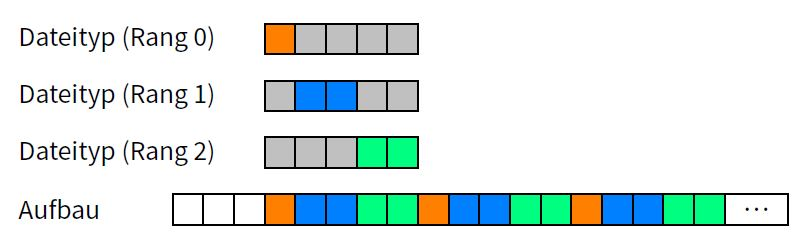
\includegraphics[width=7cm]{fig/Dateisicht.JPG}
	\caption{Dateisicht bei MPI-IO \cite{Kuhn.13.05.2016}}
	\label{fig:dateisicht}
\end{figure}
MPI-IO stellt im High-Performance-Bereich eine gute Alternative zu POSIX dar, da damit mehrere Prozesse zeitgleich auf eine Datei zugreifen bzw. in diese schreiben k\"onnen. Die popul\"arste Implementierung von MPI-IO ist ROMIO. MPI-IO bildet dar\"uber hinaus die Basis vieler IO-Systeme wie bspw. HDF.\cite{Corbett.1995}\cite{Kuhn.13.05.2016}
